\documentclass{article}
\usepackage{…/HBSuerDemir}
\usepackage{graphicx}
\usepackage{wrapfig}
\begin{document}
    \hPage{b2p1/240} %page number
    We have obtained K when the plane curve $\Gamma$ is given in vector or cartesian form. Now, for a \underline{parametric curve}
    \begin{center}
        $\Gamma : x=x(t), y=y(t),$\\
    \end{center}
    setting
    \begin{center}
        $y'=\dot y/\dot x,$ $y''=\frac{d}{dx}$   $\frac{\ddot y \dot x - \dot y \ddot x}{{\dot x}^2}$ $\frac{1}{\dot x}$,\\
    \end{center}
    in $K=y''/(1+{y'}^2)^{3/2}$, we have 
    \begin{center}
        $K=\frac{ \dot x \ddot y - \ddot x \dot y }{({\dot x}^2+{\dot y}^2)^{3/2}}$\\
    \end{center}
    
    When $\Gamma$ is given in \underline{polar form}:
    \begin{center}
        $\Gamma$: $r=f(\theta)$ or $x=r \cos\theta$, $y=r\sin\theta$,\\
    \end{center}
    computing $\dot x, \dot y, \ddot x, \ddot y$ and setting in above formulas one gets
    \begin{center}
        $K=\frac{r^2+{2r'}^2-rr''}{(r^2+{r'}^2)^{3/2}}$\\
    \end{center}
    which can also be obtained from $K=dx/ds$ where $\alpha=\psi+\theta$ and $\psi=\arctan\frac{r}{r'}$\\
    
    \underline{Circle of curvature:}\\
    
    \begin{wrapfigure}{r}{0.25\textwidth} %this figure will be at the right
        \centering
        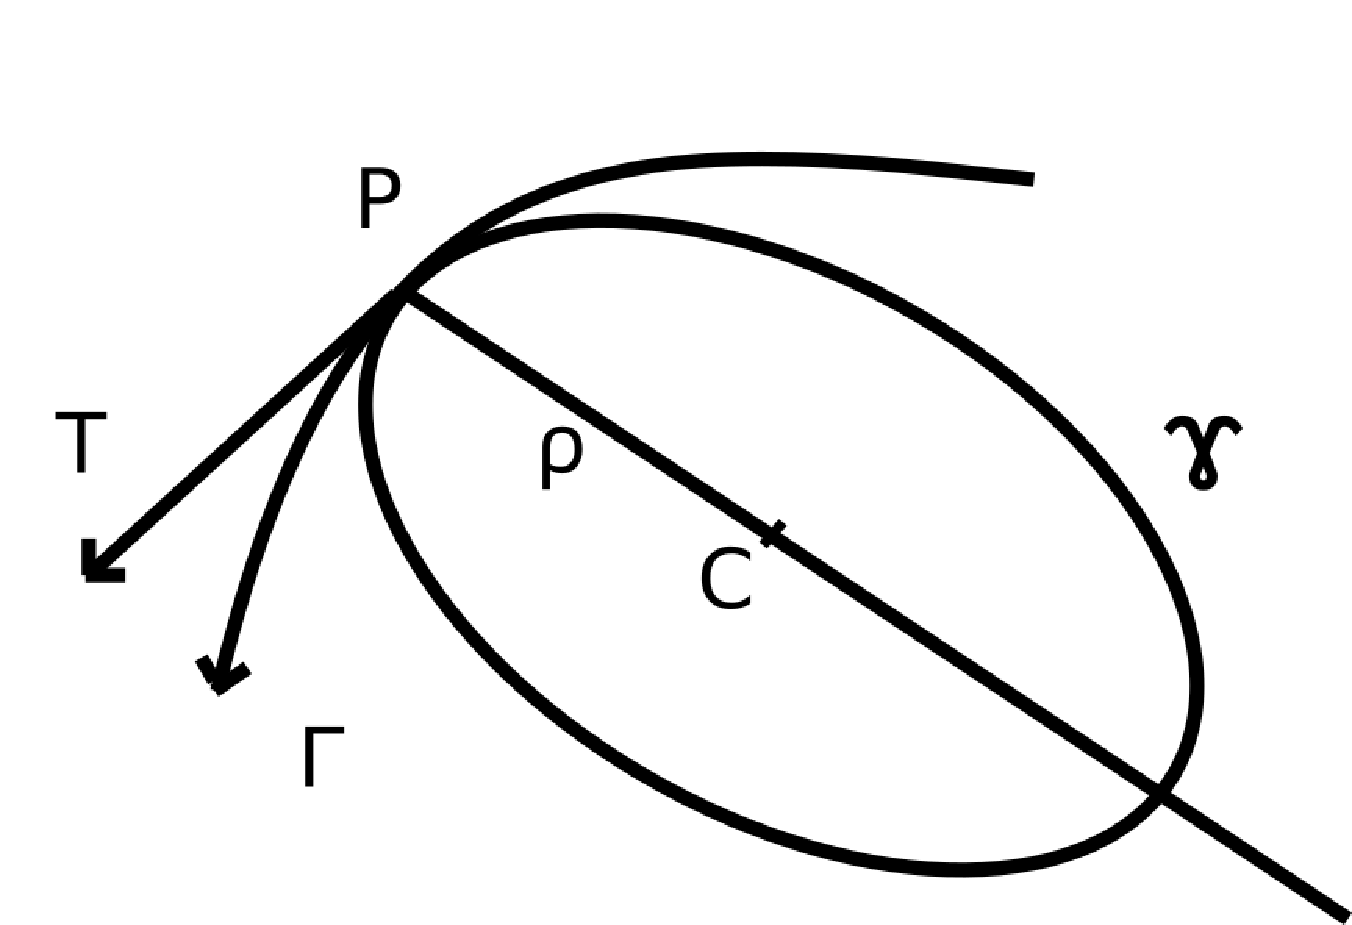
\includegraphics[width=0.3\textwidth]{images/b2p1-240-fig01.pdf}
    \end{wrapfigure}
    The circle of curvature of a curve $\Gamma$ at a point P of it, is the limiting circle of the circle passing through P and two nearby points Q, R when $Q\rightarrow P$, $R\rightarrow P$.\\
    
    It can be shown that the circle center at $C=P+\varrho N$ and radius $\varrho$ is the circle of curvature $\gamma$ at P (in 2- or 3- space). $\gamma$ lies in the oscuating plane at P since it is tangent to $\Gamma$. (or the tangent vector T) and center is on principal normal.
\end{document}